\documentclass[11pt, a4paper, twoside]{article}   	% use "amsart" instead of "article" for AMSLaTeX format

\usepackage{geometry}                		% See geometry.pdf to learn the layout options. There are lots.
\usepackage{pdfpages}
\usepackage{caption}
\usepackage{minted}
\usepackage[german]{babel}			% this end the next are needed for german umlaute
\usepackage[utf8]{inputenc}
\usepackage{color}
\usepackage{graphicx}
\usepackage{titlesec}
\usepackage{fancyhdr}
\usepackage{lastpage}
\usepackage{hyperref}
\usepackage[autostyle=false, style=english]{csquotes}
\usepackage{mathtools}
\usepackage{tabularx}
% http://www.artofproblemsolving.com/wiki/index.php/LaTeX:Symbols#Operators
% =============================================
% Layout & Colors
% =============================================
\geometry{
   a4paper,
   total={210mm,297mm},
   left=20mm,
   right=20mm,
   top=20mm,
   bottom=30mm
 }	

\definecolor{myred}{rgb}{0.8,0,0}
\definecolor{mygreen}{rgb}{0,0.6,0}
\definecolor{mygray}{rgb}{0.5,0.5,0.5}
\definecolor{mymauve}{rgb}{0.58,0,0.82}

\setcounter{secnumdepth}{4}


% the default java directory structure and the main packages
\newcommand{\srcDirBunnies}{../src/SolutionUebung1/MetaProgramming}
\newcommand{\imageDir}{images}
% =============================================
% Code Settings
% =============================================
\newenvironment{code}{\captionsetup{type=listing}}{}
\newmintedfile[cppSourceFile]{cpp}{
	linenos=true, 
	frame=single, 
	breaklines=true, 
	tabsize=2,
	numbersep=5pt,
	xleftmargin=10pt,
	baselinestretch=1,
	fontsize=\footnotesize
}
\newmintinline[inlineCpp]{cpp}{}
\newminted[cppSource]{cpp}{
	breaklines=true, 
	tabsize=2,
	autogobble=true,
	breakautoindent=false
}

\newcommand{\xvdash}[1]{%
  \vdash^{\mkern-10mu\scriptscriptstyle\rule[-.9ex]{0pt}{0pt}#1}%
}

% =============================================
% Page Style, Footers & Headers, Title
% =============================================
\title{Übung 3}
\author{Thomas Herzog}

\lhead{Übung 3}
\chead{}
\rhead{
\includegraphics[scale=0.10]{FHO_Logo_Students.jpg}}

\lfoot{S1610454013}
\cfoot{}
\rfoot{ \thepage / \pageref{LastPage} }
\renewcommand{\footrulewidth}{0.4pt}
% =============================================
% D O C U M E N T     C O N T E N T
% =============================================
% =============================================
% 2016.10.13: 1 
% 2016.10.14: 2
% =============================================
\pagestyle{fancy}
\begin{document}
\setlength{\headheight}{15mm}
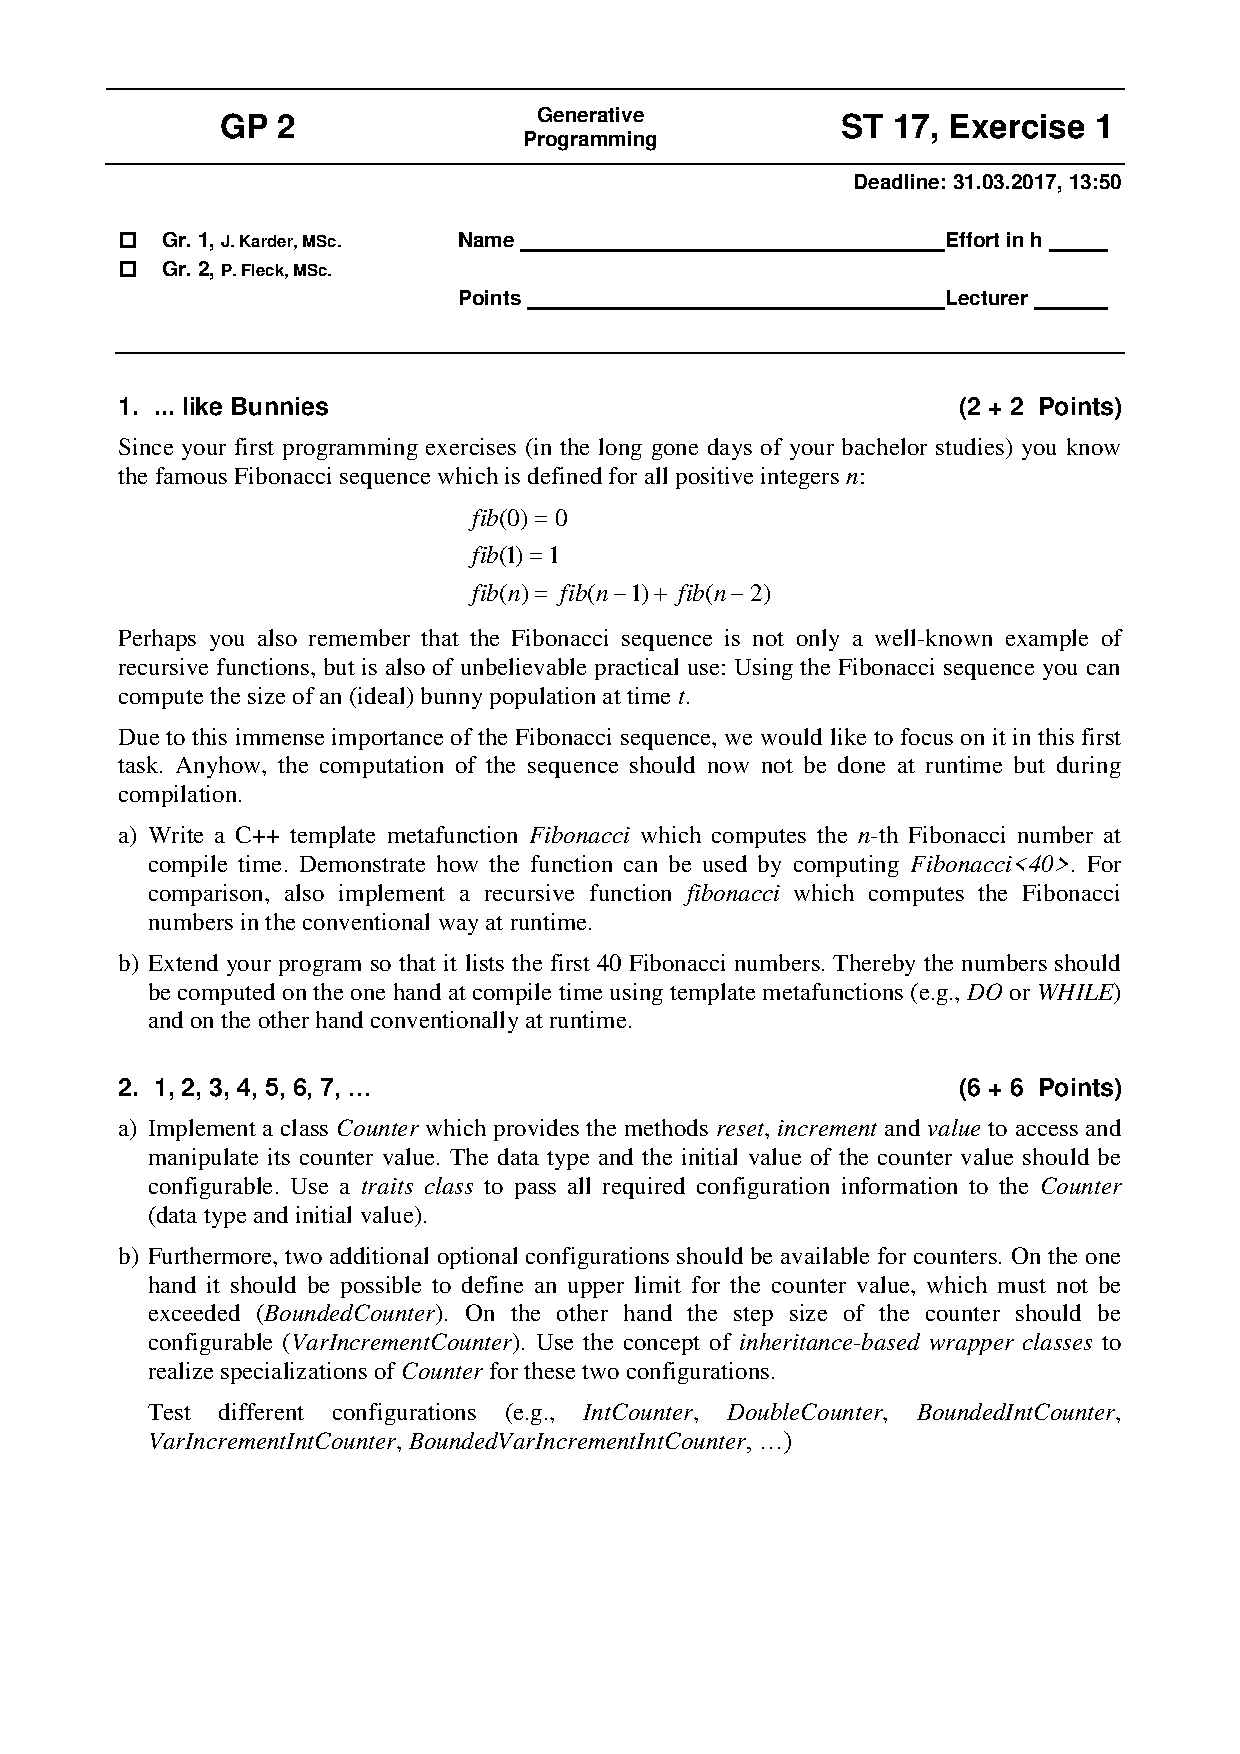
\includepdf[pages={1,2}]{GP_A01.pdf}

\section{... like Bunnies}
\subsection{Lösungsidee}
Die Implementierungen der Aufgabe \emph{like Buniies} wird in drei Dateien aufgeteilt.
\begin{itemize}
	\item fibonacci.hpp
	\item statement.hpp
	\item main.cpp
\end{itemize}
Die Berechnung der Fibonacci-Folge wird über eine rekursive Funktion implementiert, die dazu verwendet wird die Berechnung zur Laufzeit zu durchzuführen. Es wird ein Template implementiert, welches die Fibonacci-Folge zur Compile-time berechnet. Es werden zwei partielle Ausprägungen des Templates implementiert und zwar für die Werte 0 und 1. 0 damit die Instanziierung der Templates ein definiertes Ende hat und zusätzlich eine partielle Ausprägung für 1, da die Fibonacci-Folge wie folgt definiert ist $fib(n) = fib(n-1) + fib(n-1)$. 
\newline
\newline
Für die Berechnung der Fibonacci-Folge über DO-IF-Template-Metafunctions, die zur Compile-Time evaluiert werden, wird ein Template für die Berechnung der Fibonacci-Folge implementiert, sowie ein Template für die Condition, welche entscheidet wann die Berechnung fertig ist. Um das aktuelle n im Template zu speichern wird folgende Anweisung verwendet \emph{enum \{ current = n \}}. Das gespeicherte n als current wird von der \emph{FibonacciCondition} benötigt um zu entscheiden, wann die Berechnung fertig ist.
\newline
\newline
Die DO-IF-Statement Templates werden in der Datei statement.hpp implementiert. Für das IF-Template wird zusätzlich ein partielles Template für den boolschen Wert false implementiert. Das DO-Template erwartet sich zwei Typparameter \emph{Statement} und \emph{Condition}, wobei \emph{Statement} eine einfach verkettete Liste von \emph{Statements} darstellt, wobei das nächste \emph{Statement} über \emph{Statement:NEXT} verfügbar ist.
\newpage

\begin{code}
	\caption{fibonacci.hpp}
	\cppSourceFile{\srcDirBunnies/fibonacci.hpp}
	\label{src:fibonacci-hhp}
\end{code}
\ \newpage

\begin{code}
	\caption{statement.hpp}
	\cppSourceFile{\srcDirBunnies/statement.hpp}
	\label{src:statement-hhp}
\end{code}
\ \newpage

\begin{code}
	\caption{main.cpp}
	\cppSourceFile{\srcDirBunnies/main.cpp}
	\label{src:main-cpp}
\end{code}

\begin{figure}
	\centering
	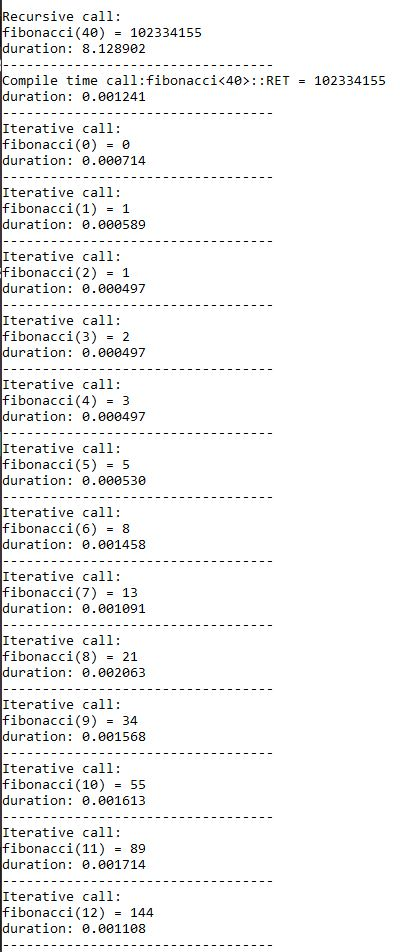
\includegraphics[scale=0.9]{\imageDir/bunnies1.JPG}
	\caption{Test Teil 1}
	\label{fig:bunnies-1}
\end{figure}

\begin{figure}
	\centering
	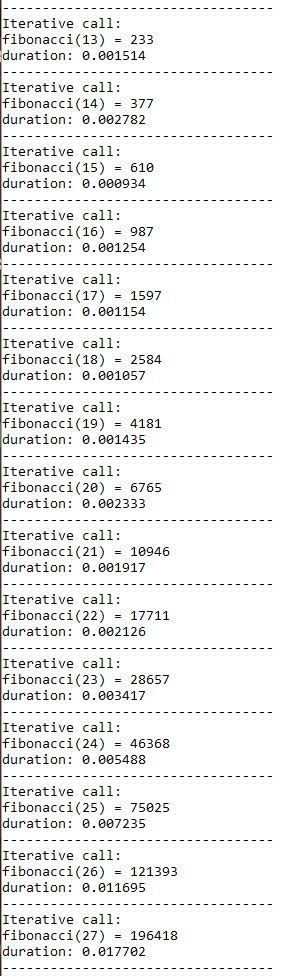
\includegraphics[scale=0.9]{\imageDir/bunnies2.JPG}
	\caption{Test Teil 2}
	\label{fig:bunnies-2}
\end{figure}

\begin{figure}
	\centering
	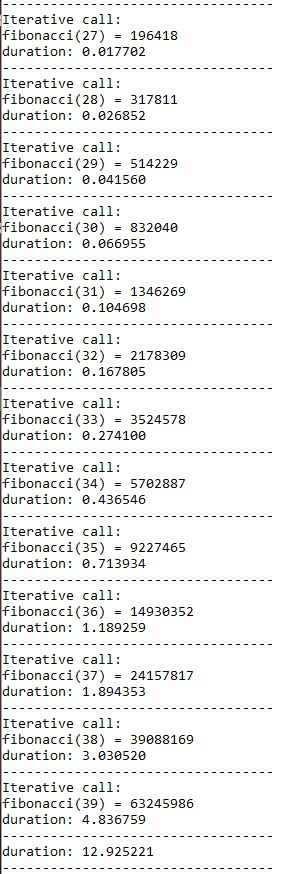
\includegraphics[scale=0.9]{\imageDir/bunnies3.JPG}
	\caption{Test Teil 3}
	\label{fig:bunnies-3}
\end{figure}

\begin{figure}
	\centering
	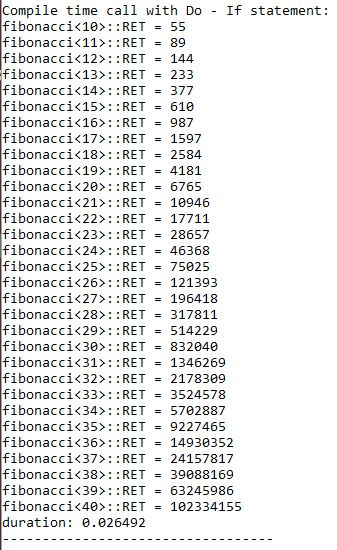
\includegraphics[scale=0.9]{\imageDir/bunnies4.JPG}
	\caption{Test Teil 4}
	\label{fig:bunnies-4}
\end{figure}
\ \newpage

\section{1, 2, 3, 4, 5, 6, ...}
\subsection{Lösungsidee}


\end{document}